\chapter{基于模型的方法计算$\CTL$下的遗忘}\label{chapter05}

{\em
	遗忘理论与均匀插值是一对对偶概念,已有研究表明$\CTL$不具有均匀插值性质~\cite{Maksimova:JANCL:1991},这就表明$\CTL$中的遗忘理论不是封闭的\footnote{对于给定的逻辑语言${\cal L}$和该语言上的操作${\cal O}$,若$\cal O$作用到$\cal L$中的元素后得到的结果仍然在$\cal L$中,则称$\cal O$在$\cal L$下是封闭的。}。
	此时,探索$\CTL$下遗忘理论封闭的情形对深入引用遗忘理论有重要意义。
	为此,本章首先提出有限初始$\MPK$-结构的特征公式;其次,表明$\CTL$公式的遗忘结果在此情形下可以表示成其模型的特征公式的吸取;最后,提出一种基于模型的方法计算遗忘,且探索了如何使用遗忘计算最弱充分条件和知识更新。
}

\section{引言}\label{sec:chapter06_introduction}
%系统模型通常是有限的
%小模型理论,公式的长度有限
%描述数(特征数)来区分同意结构内那些状态在一定程度上是相同的,如果超过这个度,肯定不同。此时,就可以使用CTL公式来描述这些状态及其关系。
%描述forgetting的四个规则。

计算树逻辑是由Clarke和Emerson提出的一种分支时间时序逻辑,它能很好的描述并发系统的一些性质。
Emerson和Halpern证明$\CTL$具有小模型属性:如果一个公式是可满足的,那么它在一个小的有限模型下是可满足的~\cite{DBLP:journals/jcss/EmersonH85}。
具体说来,对于给定的$\CTL$公式$\varphi$,如果公式的长度\footnote{给定公式$\varphi$,出现在该公式里的符号的个数为公式的长度,记为$|\varphi|$。}为$n$(记为:$|\varphi| = n$),则存在一个状态数为$n8^n$的初始$\MPK$-结构$(\Hm,s_0)$使得$(\Hm,s_0)\models \varphi$。

此外,现实情况下能处理的系统都是有限的,且在某一固定环境下所涉及到的原子命题是有限的。因此,在这部分讨论一种约束的$\CTL$,即:(1)出现在$\CTL$公式中的原子命题的个数是有限的(即$\Ha$是有限的);(2)初始结构的状态空间$S$是一个有限的固定状态空间${\cal S}=\{b_1,\ldots,b_m\}$的子集(即$S \subseteq {\cal S}$),且使得对于任意约束长度的$\CTL$公式$\varphi$,若$\varphi$是可满足的,则存在一个初始$\MPK$-结构$(\Hm,s_0)$使得$(\Hm,s_0)\models \varphi$且其状态空间是${\cal S}$的子集。由此可见,在这种情形下只有有限个初始结构应该被考虑。

下文将表明在这一约束条件下$\CTL$中的遗忘是封闭的。

本章其余部分组织如下:首先,第\ref{sec:chapter06_system_model}节介绍本章的基本定义、系统模型,提出研究问题。其次,第\ref{sec:chapter06_our_scheme}节阐述本章中提出的优化模型和ORRP方案。进一步,第\ref{sec:chapter06_privacy_utility_analysis}节给出所提方案在理论上的性能分析。随后,第\ref{sec:chapter05-experiment}节给出真实数据集上的实验结果。最后,在第\ref{sec:chapter05-conclusion}节中进行本章工作总结。

\section{描述初始$\MPK$-结构}\label{sec:chapter06_chaIntC}
本节介绍与一个初始$\MPK$-结构相关的$\CTL$公式——特征公式是如何得到的。
%对于一个给定的有限初始结构(状态个数和$\Ha$都是有限的),其不循环的计算树(状态不重复出现)的深度最多为其状态数的个数。
对于一个给定的初始$\MPK$-结构,其特征公式其计算树的特征公式密切相关。
为此,本节首先介绍计算树之间的$V$-互模拟关系,然后给出计算树的特征公式的定义,最后给出初始$\MPK$-结构的特征公式。

\subsection{计算树的$V$-互模拟}

为此,首先给出能够描述一定深度$n\in \mathbb{N}$的计算树之间的$V$-互模拟关系,记为$\Hb_n^V$。令$V\subseteq \Ha$是原子命题的集合,$i\in \{1,2\}$,$\Hm_i=(S_i,R_i,L_i,s_0^i)$(或$\Hm_i=(S_i,R_i,L_i,[\_]_i,s_0^i)$)是初始结构($\Ind$-Kripke结构),${\cal K}_i=(\Hm_i, s_i)$是$\MPK$-结构(或$\Ind$-结构)。$\Hb_n^V$被递归定义如下:
\begin{itemize}
	\item 若$L_1(s_1)-V=L_2(s_2)$,则$({\cal K}_1,{\cal K}_2) \in \Hb_0^V$;
	\item 对任意$n\ge 0$,若满足下面几个条件,则$({\cal K}_1,{\cal K}_2)\in \Hb_{n+1}^V$成立:
	\begin{itemize}
		\item $({\cal K}_1,{\cal K}_2) \in \Hb_0^V$;
		\item 对任意$(s_1,s_1')\in R_1$,存在$(s_2,s_2')\in R_2$使得$({\cal K}_1',{\cal K}_2') \in \Hb_n^V$;
		\item 对任意$(s_2,s_2')\in R_2$,存在$(s_1,s_1')\in R_1$使得$({\cal K}_1',{\cal K}_2') \in \Hb_n^V$。
	\end{itemize}
\end{itemize}
其中${\cal K}_i'=(\Hm_i,s_i')$。

当所谈及的原子命题的集合$V$很显然的时候,上述$\Hb_n^V$中的$V$可以省略,记为$\Hb_n$。此外,当讨论的$\Hm_i$$(i=1,2)$是显然的时候,可以使用$(s_1,s_2) \in \Hb_n$代替$((\Hm_1,s_1),(\Hm_2,s_2)) \in \Hb_n$。
此时,$V$-互模拟关系就可以定义如下:
\begin{definition}[$V$-互模拟]\label{def:V-bisimulation}
	令$V$是$\Ha$的一个子集,$i\in \{1,2\}$, ${\cal K}_1$和${\cal K}_2$是$\MPK$-结构(或$\Ind$-结构)。
	\begin{itemize}
		\item ${\cal K}_1$和${\cal K}_2$是$V$-互模拟的,当且仅当对所有的$n \ge 0$都有$({\cal K}_1, {\cal K}_2)\in \Hb_n$。若${\cal K}_1$和${\cal K}_2$是$V$-互模拟的,则记为${\cal K}_1 \lrto_V {\cal K}_2$。
		\item 对$\Hm_i$上的路径$\pi_i=(s_{i,1},s_{i,2},\dots)$,若对于任意的$j\in \mathbb{N}_{\ge 1}$\footnote{$\mathbb{N}_{\ge 1}$是大于等于1的整数的集合。}都有${\cal K}_{1,j} \lrto {\cal K}_{2,j}$,则$\pi_1 \lrto_V \pi_2$。其中${\cal K}_{i, j}=(\Hm_i, s_{i,j})$。
	\end{itemize}
\end{definition}

上述$V$-互模拟的定义是现有互模拟定义的一般化,这可以从下面几个方面来体现\footnote{在其他领域也有类似的定义,如:定义在数据库相关文献中的概念$k$-互模拟\cite{kaushik2002updates}。$k$-互模拟概念中涉及与本文$\Hb_n$类似的定义,只是其关系是从相反的方向(即:从孩子到父节点的方向)来说明的。此外,值得一提的是,本文的$V$-互模拟的概念是定义在$\MPK$-结构上的。}。
首先,当给定的$V$为空集且谈论指定的初始状态时,本文的$V$-互模拟与定义在Baier等文章里的互模拟等价(定义7.1\cite{Baier:PMC:2008})的概念一致。
其次,在同一文章里的基于状态的互模拟(定义7.7\cite{Baier:PMC:2008})是定义在给定结构的状态上的,因此与本文的$V$-互模拟(定义在结构的集合上)也不同。
最后,本文的$\Hb_n$的定义与Browne的论文中的状态等价$E_n$类似,只是后者是定义在状态上\cite{browne1988characterizing}而本文的定义在$\MPK$-结构(或$\Ind$-结构)上。


\begin{lemma}
给定原子命题集合$V\subseteq \Ha$和$\MPK$-结构,其中$i=1,2$且$\Hm_i=(S_i, R_i, L_i, s_0^i)$为有限初始结构。$(s_1, s_2)\in \Hb$当且仅当$s_1 \lrto_V s_2$。
\end{lemma}
\begin{proof}
	%由于$\Hb$是${\cal K}_1$和${\cal K}_2$的约束互模拟关系,所以$(s_1, s_2)\in \Hb$。
	值得注意的是对任意的$n\geq 0$,都有$\Hb_{n+1} \subseteq \Hb_n$。又因为$\Hb_0\subseteq S_1 \times S_2$ 是有限的,因而存在一个数$k$使得$\Hb_{k+1}=\Hb_k = \Hb$。
	
	(1)证明若$(s_1, s_2)\in \Hb$则$s_1 \lrto_V s_2$。
	显然,$(s_1, s_2)\in \Hb$。所以,只需要证明$\Hb$是$\Hm_1$和$\Hm_1$之间的一个$V$-互模拟关系。
	下面证明对任意的$r_1\in S_1$和$r_2\in S_2$,$(r_1,r_2) \in \Hb$当且仅当
	\begin{itemize}
		\item[](a) $L_1(r_1)-V = L_2(r_2)-V$;
		\item[](b) $\forall w_1\in S_1$, if $(r_1, w_1)\in R_1$, then $\exists w_2 \in S_2$ s.t. $(r_2,w_2) \in R_2$ and $(w_1, w_2) \in \Hb$; and 
		\item[](c) $\forall w_2\in S_2$, if $(r_2, w_2)\in R_2$, then $\exists w_1 \in S_1$ s.t. $(r_1,w_1) \in R_1$ and $(w_1, w_2)\in \Hb $.
	\end{itemize}

	$(\Rto)$ $(r_1,r_2) \in \Hb$\\
	$\Rto$ $\forall n\geq 0$,$(r_1,r_2)\in \Hb_n$\\
	$\Rto$ $(r_1,r_2)\in \Hb_0$且$\forall n > 0$,$(r_1,r_2)\in \Hb_n$\\
	$\Rto$ $L_1(r_1)-V = L_2(r_2)-V$ (因此,(a)成立),
	
	且$\forall n\geq 0$,$(r_1,r_2)\in \Hb_{n+1}$意味着下面几点成立:
	\begin{itemize}
		\item $L_1(r_1)-V = L_2(r_2)-V$;
		\item $\forall w_1 \in S_1$,若$(r_1, w_1)\in R_1$,则$\exists w_2 \in S_2$使得$(r_2,w_2) \in R_2$且$(w_1, w_2) \in \Hb_n$;且
		\item $\forall w_2\in S_2$,若$(r_2, w_2)\in R_2$,则$\exists w_1 \in S_1$使得$(r_1,w_1) \in R_1$且$(w_1, w_2)\in \Hb_n$。
	\end{itemize}
	
	因为存在一个数$k$使得$\Hb_{k+1}=\Hb_k = \Hb$,所以对这样的$k$有$(r_1,r_2)\in \Hb_{k+1}$使得:
	\begin{itemize}
		\item $L_1(r_1)-V = L_2(r_2)-V$;
		\item $\forall w_1 \in S_1$,若$(r_1, w_1)\in R_1$,则$\exists w_2 \in S_2$使得$(r_2,w_2) \in R_2$且$(w_1, w_2) \in \Hb_k$\\
		$\Rto$ $\forall w_1 \in S_1$,若$(r_1, w_1)\in R_1$,则$\exists w_2 \in S_2$使得$(r_2,w_2) \in R_2$且$(w_1, w_2) \in \Hb$ (因此,(b)成立)。
		\item $\forall w_2\in S_2$,若$(r_2, w_2)\in R_2$,则$\exists w_1 \in S_1$使得$(r_1,w_1) \in R_1$且$(w_1, w_2)\in \Hb_k$\\
		$\Rto$ $\forall w_2\in S_2$,若$(r_2, w_2)\in R_2$,则$\exists w_1 \in S_1$使得$(r_1,w_1) \in R_1$且$(w_1, w_2)\in \Hb$ (因此,(c)成立)。
	\end{itemize}
	
因此,$\Hb$是$\Hm_1$和$\Hm_1$之间的一个$V$-互模拟关系。又因为$(s_1, s_2)\in \Hb$,所以$s_1 \lrto_V s_2$。

$(\Lto)$ 假定(a)、(b)和(c)成立,这里证明$(r_1, r_2)\in \Hb$,即:对于任意的$n\geq 0$都有$(r_1, r_2)\in \Hb_n$。

\begin{itemize}
	\item[(1)]  由(a)可知$(r_1, r_2) \in \Hb_0$,即:$L_1(r_1)-V = L_2(r_2)-V$。
	\item[(2)] 由(b)可知:$\forall w_1 \in S_1$,若$(r_1, w_1)\in R_1$,则 $\exists w_2 \in S_2$使得$(r_2,w_2) \in R_2$且$\forall n\geq 0$都有$(w_1, w_2) \in \Hb_n$ \\ 
	$\Rto$ $\forall w_1 \in S_1$,若$(r_1, w_1)\in R_1$,则$\exists w_2 \in S_2$使得$(r_2,w_2) \in R_2$且$\forall n > 0$都有$(w_1, w_2) \in \Hb_{n-1}$\\
	$\Rto$ $\forall n > 0$,$\forall w_1 \in S_1$,若$(r_1, w_1)\in R_1$,则$\exists w_2 \in S_2$使得$(r_2,w_2) \in R_2$且$(w_1, w_2) \in \Hb_{n-1}$。
	\item[(3)] 由(c)可知:$\forall w_2\in S_2$,若$(r_2, w_2)\in R_2$,则 $\exists w_1 \in S_1$使得$(r_1,w_1) \in R_1$且$\forall n\geq 0$都有$(w_1, w_2)\in \Hb_n$\\
	$\Rto$ $\forall w_2\in S_2$,若$(r_2, w_2)\in R_2$,则$\exists w_1 \in S_1$使得$(r_1,w_1) \in R_1$且$\forall n > 0$都有$(w_1, w_2)\in \Hb_{n-1}$\\
	$\Rto$ $\forall n > 0$,$\forall w_2\in S_2$,若$(r_2, w_2)\in R_2$,则$\exists w_1 \in S_1$使得$(r_1,w_1) \in R_1$且$(w_1, w_2)\in \Hb_{n-1}$。
\end{itemize}

因此,$\forall n > 0$有:
\begin{itemize}
	\item $(r_1, r_2) \in \Hb_0$;
	\item $\forall w_1 \in S_1$,若$(r_1, w_1)\in R_1$,则$\exists w_2 \in S_2$使得$(r_2,w_2) \in R_2$且$(w_1, w_2) \in \Hb_{n-1}$;且
	\item $\forall w_2\in S_2$,若$(r_2, w_2)\in R_2$,则$\exists w_1 \in S_1$使得$(r_1,w_1) \in R_1$且$(w_1, w_2)\in \Hb_{n-1}$。
\end{itemize}
	
所以对于任意的$n\geq 0$都有$(r_1, r_2)\in \Hb$,即:$(r_1, r_2)\in \Hb$。

(ii) 由$s_1 \lrto_V s_2$可知存在$\Hm_1$和$\Hm_1$之间的一个$V$-互模拟关系${\cal R}$使得$(s_1, s_2)\in {\cal R}$。令$\Hb={\cal R}$,显然对任意的$n\geq 0$有$(s_1,s_2)\in \Hb_n$。
	
\end{proof}

给定原子命题集合$V\subseteq \Ha$和初始结构$\Hm_i$($i = 1, 2$)。如果下面条件同时被满足,则称$\Hm_1$的计算树$\Tr_n(s_1)$和$\Hm_2$的计算树$\Tr_n(s_2)$是$V$-互模拟的(记为$({\cal M}_1,\Tr_n(s_1))\lrto_V({\cal M}_2,\Tr_n(s_2))$,简写为$\Tr_n(s_1)\lrto_V\Tr_n(s_2)$):
\begin{itemize}
	\item $L_1(s_1)- V=L_2(s_2)- V$,
	%   \item For every subtree $\Tr_{n-1}(s_i')$ of $\Tr_n(s_i)$,
	%   $\Tr_n(s_{(i \mod 2)+1})$ has a subtree $\Tr_{n-1}(s_{(i \mod 2)+1}')$ such that
	%   $\Tr_{n-1}(s_i')\lrto_V\Tr_{n-1}(s_{(i \mod 2)+1}')$.
	\item 对$\Tr_n(s_1)$的任意子树$\Tr_{n-1}(s_1')$,都存在  $\Tr_n(s_2)$的一棵子树$\Tr_{n-1}(s_2')$使得 
	$\Tr_{n-1}(s_1')\lrto_V\Tr_{n-1}(s_2')$,且
	\item 对任意$\Tr_n(s_2)$的子树$\Tr_{n-1}(s_2')$,都存在$\Tr_n(s_1)$的一棵子树$\Tr_{n-1}(s_1')$使得
	$\Tr_{n-1}(s_1')\lrto_V\Tr_{n-1}(s_2')$。
\end{itemize}

在上述定义中,当$n=0$时,只需考虑第一个条件。

\begin{proposition}\label{B_to_T}
	给定原子命题集合$V\subseteq\cal A$和$\MPK$结构$({\cal M}_i,s_i)$($i=1,2$)。
	则:
	\[(s_1,s_2)\in{\cal B}_n\mbox{当且仅当对任意的$0\le j\le n$有}
	\Tr_j(s_1)\lrto_V\Tr_j(s_2)\mbox{。}\]
\end{proposition}
\begin{proof}
	这里从下面两个方面来证明这一结论:
	
	$(\Rto)$ 这里证明“如果$(s_1, s_2) \in \Hb_n$,则对于任意的$0 \leq j \leq n$有$Tr_j(s_1) \lrto_V Tr_j(s_2)$”成立。$(s_1, s_2) \in \Hb_n$意味着$Tr_n(s_1)$和$Tr_n(s_2)$的根有同样的标签(除了$V$里的元素之外)。
	此外,对任意的$(s_1, s_{1,1}) \in R_1$,存在一个$(s_2, s_{2,1})\in R_2$使得$(s_{1,1}, s_{2,1}) \in \Hb_{n-1}$;且对任意的$(s_2, s_{2,1})\in R_2$,存在一个$(s_1, s_{1,1}) \in R_1$使得$(s_{1,1}, s_{2,1}) \in \Hb_{n-1}$。
	因此,由定义可知$Tr_1(s_1) \lrto_V Tr_1(s_2)$。递归地使用上述方法可得对任意的$0 \leq j \leq n$都有$Tr_j(s_1) \lrto_V Tr_j(s_2)$。
	
	$(\Lto)$这里证明“如果对于任意的$0 \leq j \leq n$有$Tr_j(s_1) \lrto_V Tr_j(s_2)$,则$Tr_j(s_1) \lrto_V Tr_j(s_2)$”成立。
	由$Tr_0(s_1) \lrto_V Tr_0(s_2)$可知$L(s_1) - V = L'(s_2) - V$,因而$(s_1, s_2) \in \Hb_0$。
	由$Tr_1(s_1) \lrto_V Tr_1(s_2)$可知$L(s_1) - V = L'(s_2)- V$,且对于一棵树根的任意后继状态$s$,都能找到另一棵树根的一个后继状态$s'$使得$(s, s')\in \Hb_0$。
	因此有$(s_1, s_2) \in \Hb_1$。同理可证$(s_1, s_2) \in \Hb_2$, \dots, $(s_1, s_2) \in \Hb_n$。
\end{proof}

命题~\ref{B_to_T}表明如果任意两个初始结构中的两个状态$s_1$和$s_2$能够在$\Ha-V$上相互模拟对方直到$n$步,当且仅当分别以$s_1$和$s_2$为根的计算树能在$\Ha-V$上相互模拟直到深度为$n$。
由此可知,如果同一初始结构的两个状态$s$和$s'$不是$V$-互模拟的,则存在一个数$k\in \mathbb{N}$使得分别以$s$和$s'$为根的计算树$\Tr_k(s)$和$\Tr_k(s')$不是$V$-互模拟的。
\begin{proposition}\label{pro:k}
	给定原子命题集合$V\subseteq \Ha$、初始结构$\Hm$和两个状态$s,s'\in S$。
	若$s\not\lrto_V s'$,则存在一个最小整数$k$使得$\Tr_k(s)$和$\Tr_k(s')$不是$V$-互模拟的。
\end{proposition}
\begin{proof}
	若$s\not\lrto_V s'$,则存在一个最小的数$c$使得$(s_i, s_j) \notin \Hb_c$。因此,由命题~\ref{B_to_T}可知,存在一个最小整数$m$($m \leq c$)使得$\Tr_m(s_i)$和 $\Tr_m(s_j)$不是$V$-互模拟的。令$k=m$可得上述结论。
\end{proof}

\subsection{计算树的特征公式}
由上面小节的讨论可知,$V$-互模拟可以将计算树分别开来\footnote{Similar approaches has been taken in the literature e.g., in~\cite{DBLP:conf/birthday/1997ehrenfeucht},  a class (namely, $\equiv_{\overline{k}}$-class) of structures of monadic formulas has been characterized by Hintikka formulas~\cite{hintikka1953distributive}. Another example is Yankov-Fine construction in \cite{yankov1968three}.}。本节讨论如何使用$\CTL$公式描述一棵计算树,且表明具有(或没有)$V$-互模拟关系之间的计算树的特征公式又有怎么样的关系。为此,首先给出计算树的特征公式的定义。
\begin{definition}\label{def:V:char:formula}
	给定原子命题集合$V\subseteq \Ha$、初始结构$\Hm =(S,R,L,s_0)$和状态$s\in S$。
	定义在$V$上的计算树$\Tr_n(s)$的特征公式(记为${\cal F}_V(\Tr_n(s))$,$n\geq 0$)被递归定义如下:
	\begin{align*}
		{\cal F}_V(\Tr_0(s)) &=  \bigwedge_{p \in V\cap L(s)}p
		\wedge \bigwedge_{q\in V-L(s)} \neg q,\\
		{\cal F}_V(\Tr_{k+1}(s))& = \bigwedge_{(s,s')\in R}
		\EXIST \NEXT {\cal F}_V(\Tr_k(s')) 
		\wedge 
		\ALL \NEXT \bigg( \bigvee_{(s,s')\in R} {\cal F}_V(\Tr_k(s')) \bigg) \wedge {\cal F}_V(\Tr_0(s)) \hbox{ ($k\ge 0$)。}
	\end{align*}
\end{definition}

由定义~\ref{def:V:char:formula}可知,计算树的特征公式从三个方面展示了计算树的信息:(1)只考虑$V$中的原子命题;(2)突出了树节点的内容,即:对于任意原子命题$p\in V$,若$p$在节点的标签中,则其正出现在特征公式中,否则负出现在特征公式中;(3)公式中的时序算子表示了状态之间的转换关系。
通俗地讲,${\cal F}_V(\Tr_0(s))$表明了节点$s$的在$V$上的内容;$\EXIST \NEXT$的合取部分和$\ALL \NEXT$部分保证以$s$的每个直接后继状态$s'$为根深度为$k$的计算树都有一个$\CTL$公式来描述。

下面的结论表明,若两个计算树是$V$-互模拟的,则他们在$V$上的特征公式是逻辑等价的。
\begin{lemma}\label{lem:Vb:TrFormula:Equ}
	给定原子命题集合$V\subseteq \Ha$、初始结构$\Hm=(S,R,L,s_0)$和$\Hm'=(S',R',L',s_0')$、$s\in S$、$s'\in S'$且 $n\ge 0$。若$\Tr_n(s) \lrto_{\overline V} \Tr_n(s')$,则${\cal F}_V(\Tr_n(s)) \equiv {\cal F}_V(\Tr_n(s'))$。
\end{lemma}
\begin{proof}
	通过归纳计算树的深度$n$来证明。
	
	\textbf{基始($n=0$):} 对任意的$s_x\in S$和$s_x' \in S'$,若$\Tr_0(s_x) \lrto_{\overline V} \Tr_0(s_x')$,则由$L(s_x) - \overline V = L'(s_x') - \overline V$可知${\cal F}_V(\Tr_0(s_x)) \equiv {\cal F}_V(\Tr_0(s_x'))$。
	
	\textbf{归纳步($n>0$):} 假设对任意的$0\leq m \leq n$若$\Tr_m(s) \lrto_{\overline V} \Tr_m(s')$,则${\cal F}_V(\Tr_m(s)) \equiv {\cal F}_V(\Tr_m(s'))$。
	这里要证明若$\Tr_{n+1}(s) \lrto_{\overline V} \Tr_{n+1}(s')$,则${\cal F}_V(\Tr_{n+1}(s)) \equiv {\cal F}_V(\Tr_{n+1}(s'))$。
	
	由归纳假设可知,对任意的$k=m$、$s_k\in S$ 和$s_k'\in S'$,若$\Tr_{n-k}(s_k) \lrto_{\overline V} \Tr_{n-k}(s_k')$,则${\cal F}_V(\Tr_{n-k}(s_k)) \equiv {\cal F}_V(\Tr_{n-k}(s_k'))$。
	因此,要证原结论成立,只需要证明若$\Tr_{n-k+1}(s_{k-1}) \lrto_{\overline V} \Tr_{n-k+1}(s_{k-1}')$,则${\cal F}_V(\Tr_{n-k+1}(s_{k-1})) \equiv {\cal F}_V(\Tr_{n-k+1}(s_{k-1}'))$。其中,$(s_{k-1},s_k)\in R$且$(s_{k-1}',s_k')\in R'$。
	显然,由计算树的特征公式可知:
	\begin{align*}
		{\cal F}_V(\Tr_{n-k+1}(s_{k-1})) &  =
		\left(\bigwedge_{(s_{k-1},s_k)\in R}
		\EXIST \NEXT {\cal F}_V(\Tr_{n-k}(s_k))\right)
		\wedge \\
		&\ALL \NEXT\left(\bigvee_{(s_{k-1},s_k)\in R}
		{\cal F}_V(\Tr_{n-k}(s_k) )\right)
		\wedge {\cal F}_V(\Tr_0(s_{k-1}))
	\end{align*}
	and
	\begin{align*}
		{\cal F}_V(\Tr_{n-k+1}(s_{k-1}')) &  =
		\left(\bigwedge_{(s_{k-1}',s_k')\in R}
		\EXIST \NEXT {\cal F}_V(\Tr_{n-k}(s_k'))\right)
		\wedge \\
		&\ALL \NEXT\left(\bigvee_{(s_{k-1}',s_k')\in R}
		{\cal F}_V(\Tr_{n-k}(s_k') )\right)
		\wedge {\cal F}_V(\Tr_0(s_{k-1}')).
	\end{align*} 

	又因为$\Tr_{n-k+1}(s_{k-1})$ $\lrto_{\overline V} \Tr_{n-k+1}(s_{k-1}')$,所以对任意的$(s_{k-1}, s_k) \in R$存在$(s_{k-1}', s_k') \in R'$使得$\Tr_{n-k}(s_k) \lrto_{\overline V} \Tr_{n-k}(s_k')$,且对任意的$(s_{k-1}', s_k') \in R'$存在$(s_{k-1}, s_k) \in R$使得$\Tr_{n-k}(s_k) \lrto_{\overline V} \Tr_{n-k}(s_k')$。
	因此,由归纳假设可知${\cal F}_V(\Tr_{n-k+1}(s_{k-1})) \equiv {\cal F}_V(\Tr_{n-k+1}(s_{k-1}'))$。
\end{proof}

此外,对于初始结构$\Hm$上的状态$s$和$s'$,若$(\Hm,s)$是定义在$V$上的根为$s'$深度为$n$的计算树的特征公式,则$s$和$s'$至少属于$\Hb_n$,即:$s$和$s'$能想互模拟至少到第$n$层深度。

\begin{lemma}\label{Bn:to:Tn}
	令$V\subseteq \Ha$、$\Hm=(S, R, L,s_0)$、$\Hm'=(S', R', L',s_0')$、$s\in S$、$s'\in S'$且$n\ge 0$,则:
	\begin{itemize}
		\item[(i)] $({\cal M},s)\models{\cal F}_V(\Tr_n(s))$;
		\item[(ii)] 若$({\cal M},s)\models{\cal F}_V(\Tr_n(s'))$,则
		$\Tr_n(s) \lrto_{\overline V} \Tr_n(s')$。
	\end{itemize}
\end{lemma}
\begin{proof}
	(i) \textbf{基始($n=0$):}从树的特征公式定义可知${\cal F}_V(\Tr_0(s))$是显然的。

	\textbf{归纳步($n>0$):} 假设对任意的$k\geq 0$,$({\cal M},s)\models{\cal F}_V(\Tr_k(s))$,下面证明$({\cal M},s)\models{\cal F}_V(\Tr_{k+1}(s))$,即:
	\begin{equation*}
		({\cal M},s)\models \left(\bigwedge_{(s,s')\in R}
		\EXIST \NEXT T(s')\right)
		\wedge \ALL \NEXT\left(\bigvee_{(s,s')\in R}
		T(s')\right)
		\wedge {\cal F}_V(\Tr_0(s)).
	\end{equation*}
	其中$T(s') ={\cal F}_V(\Tr_k(s'))$。 
	由基始可知$({\cal M},s)\models {\cal F}_V(\Tr_0(s))$。
	由归纳假设可知,对任意的$(s,s') \in R$有$({\cal M}, s') \models {\cal F}_V(\Tr_k(s'))$。因此有$({\cal M},s)\models \EXIST \NEXT {\cal F}_V(\Tr_k(s')$,从而$({\cal M},s)\models \bigwedge_{(s,s')\in R}
	\EXIST \NEXT {\cal F}_V(\Tr_k(s'))$。
	
	同理,对任意的$(s,s') \in R$都有$({\cal M}, s') \models \bigvee_{(s,s')\in R} {\cal F}_V(\Tr_k(s') )$。因此,
	$$({\cal M},s)\models \ALL \NEXT\left(\bigvee_{(s,s')\in R}
	{\cal F}_V(\Tr_k(s') )\right)$$
	
	从而可知对任意的$n\geq 0$,$({\cal M},s)\models{\cal F}_V(\Tr_n(s))$。
	
	
	
	(ii) \textbf{基始($n=0$):}若$(\Hm, s)  \models {\cal F}_V(\Tr_0(s'))$ ,则$L(s) - \overline V = L'(s') - \overline V$。因此$\Tr_0(s) \lrto_{\overline V} \Tr_0(s')$。
	
	\textbf{归纳步($n>0$):} 假定若$({\cal M},s)\models{\cal F}_V(\Tr_{n-1}(s'))$,则$\Tr_{n-1}(s) \lrto_{\overline V} \Tr_{n-1}(s')$。下面证明若$({\cal M},s)\models{\cal F}_V(\Tr_n(s'))$,则
	$\Tr_n(s) \lrto_{\overline V} \Tr_n(s')$。
	
	\begin{itemize}
		\item[(a)] 由基始知$L(s) - \overline V = L'(s') - \overline V$;
		\item[(b)] 因为$(\Hm, s) \models {\cal F}_V(\Tr_n(s'))$,所以$(\Hm, s) \models \ALL \NEXT\left(\bigvee_{(s',s_1')\in R}{\cal F}_V(\Tr_{n-1}(s_1') )\right)$。由此,对于任意的$(s, s_1) \in R$,存在$(s', s_1') \in R'$使得$(\Hm, s_1) \models {\cal F}_V(\Tr_{n-1}(s_1') )$。由归纳假设可知$\Tr_{n-1}(s_1) \lrto_{\overline V} \Tr_{n-1}(s_1')$。即:$\forall (s, s_1) \in R$,$\exists (s', s_1') \in R'$使得$\Tr_{n-1}(s_1) \lrto_{\overline V} \Tr_{n-1}(s_1')$。
		\item[(c)] 因为$(\Hm, s) \models {\cal F}_V(\Tr_n(s'))$,所以$(\Hm, s) \models  \bigwedge_{(s',s_1')\in R'} \EXIST \NEXT {\cal F}_V(\Tr_{n-1}(s_1'))$。由此,对于任意的$(s',s_1')\in R'$,存在$(s,s_1)\in R$使得$(\Hm, s_1) \models {\cal F}_V(\Tr_{n-1}(s_1')$。由归纳假设可知$\Tr_{n-1}(s_1) \lrto_{\overline V} \Tr_{n-1}(s_1')$。即:$\forall (s',s_1')\in R'$,$\exists (s,s_1)\in R$使得$\Tr_{n-1}(s_1) \lrto_{\overline V} \Tr_{n-1}(s_1')$。
	\end{itemize}
\end{proof}

%在引理~\ref{lem:Vb:TrFormula:Equ}中,若令$s'=s$

\subsection{初始$\MPK$-结构的特征公式}
由$V$-互模拟的定义和命题~\ref{pro:k}可以自然地得到一个$V$-互模拟的补概念——$V$-可区分的。
特别地,在命题~\ref{pro:k}中,若初始结构$\Hm$的两个状态$s$和$s'$不是$\overline{V}$-互模拟的(即:$s\not\lrto_{\overline{V}} s'$),则称$s$和$s'$是\emph{$V$-可区分的}。
且用$\dis_V({\cal M},s,s',k)$表示状态$s$和$s'$在命题~\ref{pro:k}中所说的最小数$k$下是$V$-可区分的。
正如下文所说,$V$-可区分这一概念是定义初始$\MPK$-结构的特征公式重要概念。

此外,对于给定的初始结构$\Hm$和原子命题集合$V$,若在$\Hm$中存在两个状态$s$和$s'$是$V$-可区分的,则称$\Hm$是$V$-可区分的。
而对于一个$V$-可区分的初始结构$\Hm$,存在一个一个最小的数$k$使得对于该结构上的任意两个状态$s$和$s'$,若$s$和$s'$是可区分的,则$(s,s')\not \in \Hb_k$。本文称这样的数为$\Hm$关于$V$的\emph{特征数},记为$ch({\cal M},V)$,其定义如下:
\[ch({\cal M},V)=
\left\{
\begin{array}{ll}
	\max\{k\mid s,s'\in S \text{ 且 }\dis_V({\cal M},s,s',k)\}, \qquad \hbox{${\cal M}$ 是 $V$-可区分的;} \\
	\min\{k\mid {\cal B}_{k}={\cal B}_{k+1}, k\ge 0\}, \ \ \ \quad  \qquad \qquad \qquad \hbox{否则。}
\end{array}
\right.
\]

由$ch({\cal M},V)$定义可知,对于任意的$\Hm$和$V$,$ch({\cal M},V)$总是存在的,这体现在两个方面:(1)若$\Hm$是$V$-可区分的,存在两个状态$s$和$s'$是$V$-可区分的,由命题~\ref{pro:k}可知,存在一个数$k$使得$\dis_V({\cal M},s,s',k)$成立;(2)若对于任意$k\geq 0$和$\Hm$上的两个状态$s$和$s'$都有$(s,s')\in \Hb_k$且$\Hb_k =\Hb_{k+1}$,则$ch({\cal M},V)=0$。

非形式化地说,特征数$c=ch({\cal M},V)$将$\Hm$上的状态分为两大类:第一类中的任意两个状态$s$和$s'$是$V$-可区分的,且$(s,s')\not \in \Hb_c$;第二类中状态都是$V$-不可区分的。这也在计算树的特征公式上:

\begin{lemma}\label{div_s}
	令$V\subseteq \Ha$、$\Hm=(S,R,L,s_0)$、$k={ch({\cal M},V)}$且$s\in S$,则
	%There is a formula $\phi$ such that
	\begin{itemize}
		\item[(i)] $(\Hm, s)\models {\cal F}_V(\Tr_k(s))$;
		\item[(ii)] 对任意的$s'\in S$,$({\cal M},s) \lrto_{\overline V} ({\cal M},s')$
		当且仅当$({\cal M},s')\models{\cal F}_V(\Tr_k(s))$。
	\end{itemize}
\end{lemma}
\begin{proof}
	(i) 这由引理~\ref{Bn:to:Tn}易知。
	
	(ii) 令$\phi = {\cal F}_V(\Tr_k(s))$($k$为$\Hm$关于$V$的特征数)。由(i)知 $(\Hm, s) \models \phi$,从而对任意的$s' \in S$,若$s \lrto_{\overline V} s'$,由定理~\ref{thm:V-bisimulation:EQ}和$\IR(\phi, \Ha - V)$知$(\Hm, s') \models \phi$。
	
	假定$(\Hm, s')\models \phi$。若$s \nleftrightarrow_{\overline V} s'$,则$\Tr_k(s) \not \lrto_{\overline V} \Tr_k(s')$,因而由引理~\ref{Bn:to:Tn}可知$(\Hm, s')\not \models \phi$,这与假定矛盾。
\end{proof}

由此,可定义初始$\MPK$-结构的特征公式如下。

\begin{definition}[特征公式]
	给定原子命题集合$V\subseteq\cal A$he和初始\MPK-结构${\cal K}=({\cal M},s_0)$,其中$c=ch({\cal M},V)$。对任意$\Hm$上得状态$s' \in S$,记$T(s') = {\cal F}_V(\Tr_c(s'))$。
	则$\cal K$关于$V$的{\em 特征公式} ${\cal F}_V({\cal K})$为:
	\[T(s_0) \text{ } \wedge \bigwedge_{s\in S}\ALL \GLOBAL\left(
	T(s) \rto
	\bigwedge_{(s,s')\in R}
	\EXIST \NEXT T(s')
	\wedge
	\ALL \NEXT \bigg(\bigvee_{(s,s')\in R}T(s')\bigg)
	\right)
	\]
	
\end{definition}

有时为了凸显出初始结构及其初始状态,也把特征公式写为${\cal F}_V(\Hm, s_0)$。显然,$\IR({\cal F}_V(\Hm, s_0), \overline V)$。此外,在特征公式的定义中,使用了深度为$c$(即:特征数)的计算树的特征公式意在表明对任意$\Hm$上的两个状态$s$和$s'$,$s$和$s'$是$V$-可区分的当且仅当${\cal F}_V(\Tr_c(s))\not \equiv {\cal F}_V(\Tr_c(s'))$。特别地,$T(s_0)$确保了初始\MPK-结构的初始状态被$\CTL$公式描述;其余部分表明了结构$\Hm$上状态之间的转换关系。
下面的例子给出了计算特征公式的一般步骤:

\begin{example}[Continued from Example~\ref{ex:2}]\label{ex:4}
	考虑图~\ref{fig:K2Tree}中左边的初始$\MPK$-结构${\cal K}_2= (\Hm, s_0)$(其最初出现在图~\ref{v1uv2}中)。左边的为$\Hm$上的四棵计算树:从左到右表示以$s_0$为根、深度分别为0、1、2和3的计算树(为简化图,计算树的标签没有给出,但是每个树节点的标签可从${\cal K}_2$找到。)。令$V=\{d\}$,则 $\overline{V}=\{s, se\}$。
	
	因为$L(s_1) - \overline{V} = L(s_2) - \overline{V}$,所以有$\Tr_0(s_1) \lrto_{\overline{V}} \Tr_0(s_2)$。由于存在$(s_1, s_2)\in R$使得对任意的$(s_2, s') \in R$都有$L(s_2)- \overline V \neq L(s') - \overline V$,所以$\Tr_1(s_1) \not \lrto_{\overline{V}} \Tr_1(s_2)$。
	由此可知$s_1$和$s_2$是$V$-可区分的,且$\dis_{V}(\Hm, s_1, s_2, 1)$。
	
	 同样,我们可得到:$\dis_{ V}(\Hm, s_0, s_1, 0)$、$\dis_{V}(\Hm, s_1, s_3', 1)$、$\dis_{V}(\Hm, s_0, s_2, 0)$和$\dis_{ V}(\Hm,$ $s_0, s_3', 0)$。此外,$s_2 \lrto_{\overline V} s_3'$。因此可以计算$\Hm$关于$V$的特征数为:
	 $$ch(\Hm, V)=\max\{k\mid s,s'\in S \text{ and } \dis_{V}({\cal M},s,s',k)\} = 1.$$
	 
	  
	所以,可以由以下步骤计算${\cal K}_2$关于$V$的特征公式:
	\begin{align*}
		{\cal F}_V(\Tr_0(s_0)) &= d, \qquad \quad {\cal F}_V(\Tr_0(s_1)) = \neg d, \\
		{\cal F}_V(\Tr_0(s_2)) &= \neg d,  \qquad  {\cal F}_V(\Tr_0(s_3')) = \neg d,\\
		{\cal F}_V(\Tr_1(s_0)) &= \EXIST\NEXT \neg d \wedge \ALL\NEXT \neg d \wedge d \equiv \ALL\NEXT \neg d \wedge d, \\
		{\cal F}_V(\Tr_1(s_1)) &= \EXIST\NEXT \neg d \wedge \EXIST\NEXT \neg d  \wedge \ALL\NEXT (\neg d \vee \neg d) \wedge \neg d 
		\equiv \ALL\NEXT \neg d \wedge \neg d, \\
		{\cal F}_V(\Tr_1(s_2)) &= \EXIST\NEXT d  \wedge \ALL\NEXT d \wedge \neg d \equiv \ALL\NEXT d \wedge \neg d,\\
		{\cal F}_V(\Tr_1(s_3')) &\equiv {\cal F}_V(\Tr_1(s_2)),\\
		{\cal F}_V(\Hm, s_0)&\equiv \ALL\NEXT \neg d \wedge d \wedge \\
		& \ALL \GLOBAL(\ALL\NEXT \neg d \wedge d \rto \ALL\NEXT(\ALL\NEXT \neg d \wedge \neg d))\wedge \\
		& \ALL \GLOBAL(\ALL\NEXT \neg d \wedge \neg d \rto \ALL\NEXT(\ALL\NEXT d \wedge \neg d)) \wedge\\
		& \ALL \GLOBAL(\ALL\NEXT d \wedge \neg d \rto \ALL\NEXT(\ALL\NEXT \neg d \wedge d)).
	\end{align*}
	
	
	
	\begin{figure*}
		\centering
		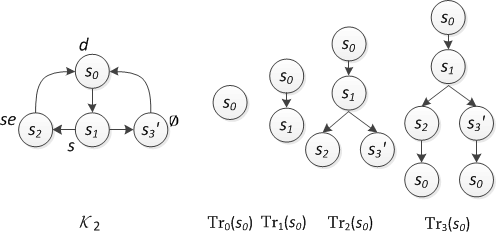
\includegraphics[width=10cm]{chapter05/NK2Tree1.png}
		\caption{左图为初始$\MPK$-结构$\mathcal{K}_2$ (源于图~\ref{v1uv2}); 右图:从左到右表示以$s_0$为根、深度分别为0、1、2和3的计算树(为简化图,计算树的标签没有给出,但是每个树节点的标签可从${\cal K}_2$找到。)}\label{fig:K2Tree}
	\end{figure*}

%\begin{figure*}[!htb]
%	\centering
%	% Requires \usepackage{graphicx}
%	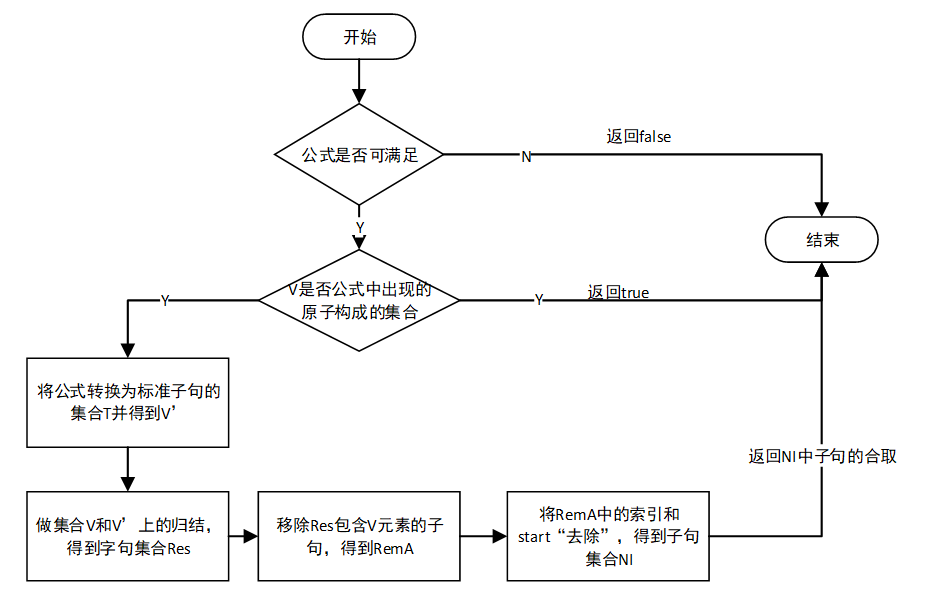
\includegraphics[width=15cm]{chapter04/frame.png}\\
%	\caption{基于归结的遗忘的主要流程图}
%	\label{Fig:chapter05:v1uv2}
%\end{figure*}

\end{example}


下面的定理表示上述定义的特征公式确实描述了一个初始\MPK-结构,此时对系统结构的操作就可转换为对其特征公式的操作,如下文将要讲的给定系统下的最弱充分条件计算。更直观地说,特征公式保持了给定初始$\MPK$-结构在原子命题集合$V$上的所有特性,即:具有$\overline{V}$-互模拟的两个初始$\MPK$-结构关于$V$的特征公式逻辑等价。

\begin{theorem}\label{CF}
	令$V\subseteq \Ha$、$\Hm=(S,R,L,s_0)$且$\Hm'=(S',R', L',s_0')$,则:
	\begin{itemize}
		\item[(i)] $(\Hm',s_0') \models {\cal F}_V({\cal M},s_0)
		\text{ 当且仅当 }
		({\cal M},s_0) \lrto_{\overline V} ({\cal M}',s_0')$;
		
		\item[(ii)] 若$s_0 \lrto_{\overline V} s_0'$则${\cal F}_V(\Hm, s_0) \equiv {\cal F}_V(\Hm', s_0')$。
	\end{itemize}
	
\end{theorem}
\begin{proof}
	(i) 令${\cal F}_V(\Hm, s_0)$为$(\Hm, s_0)$关于$V$的特征公式。显然,$\IR({\cal F}_V(\Hm, s_0), \overline V)$。为了证明上述结论成立,下面证明首先证明$(\Hm, s_0) \models {\cal F}_V(\Hm, s_0)$。
	
	令$c={ch({\cal M},V)}$,由引理~\ref{Bn:to:Tn}可知$(\Hm, s_0) \models {\cal F}_V(\Tr_c(s_0))$。下面证明特征公式里的另一部分,即:$(\Hm, s_0) \models \bigwedge_{s\in S} \ALL\GLOBAL\ G(\Hm, s)$,其中
	\[G(\Hm, s) = {\cal F}_V(\Tr_c(s)) \rto \left(\bigwedge_{(s,s_1) \in R} \EXIST \NEXT {\cal F}_V(\Tr_c(s_1))\right)\wedge \ALL \NEXT \left(\bigvee_{(s,s_1) \in R} {\cal F}_V(\Tr_c(s_1))\right).\]
	
	为此,下面证明$(\Hm, s_0) \models \ALL\GLOBAL\ G(\Hm, s)$。考虑下面两种情况:
	\begin{itemize}
		\item  若$(\Hm, s_0) \not \models {\cal F}_V(\Tr_c(s))$,显然$(\Hm, s_0) \models G(\Hm, s)$;
		\item 若$(\Hm, s_0) \models {\cal F}_V(\Tr_c(s))$:\\
		$(\Hm, s_0) \models {\cal F}_V(\Tr_c(s))$\\
		$\Rto$  $s_0 \lrto_{\overline V} s$ \hfill (引理~\ref{div_s})
		
		$\forall (s, s_1)\in R$:\\
		$(\Hm, s_1) \models {\cal F}_V(\Tr_c(s_1))$  \hfill  ($s_1 \lrto_{\overline V} s_1$)\\
		$\Rto$ $(\Hm, s) \models \bigwedge_{(s,s_1)\in R}\EXIST \NEXT {\cal F}_V(\Tr_c(s_1))$\\
		$\Rto$ $(\Hm, s_0) \models$ $\bigwedge_{(s,s_1)\in R}\EXIST \NEXT {\cal F}_V(\Tr_c(s_1))$    \qquad  ($\IR(\bigwedge_{(s,s_1)\in R}\EXIST \NEXT {\cal F}_V(\Tr_c(s_1)), \overline V)$, $s_0 \lrto_{\overline V} s$)
		
		$\forall (s, s_1) \in R$:\\
		$(\Hm, s_1) \models \bigvee_{(s, s_2)\in R}{\cal F}_V(\Tr_c(s_2))$\\
		$\Rto$ $(\Hm, s) \models \ALL \NEXT \left( \bigvee_{(s, s_2)\in R} {\cal F}_V(\Tr_c(s_2)) \right)$ \\
		$\Rto$ $(\Hm, s_0) \models$  $\ALL \NEXT \left( \bigvee_{(s, s_2)\in R} {\cal F}_V(\Tr_c(s_2)) \right)$   \hfill   ($\IR(\ALL \NEXT \left( \bigvee_{(s, s_2)\in R} {\cal F}_V(\Tr_c(s_2)) \right), \overline V)$, $s_0 \lrto_{\overline V} s$)\\
		$\Rto$ $(\Hm, s_0) \models G(\Hm, s)$。\\
		% where $s_i$ and $s_j$ are the successors of $s$.
	\end{itemize}
	
	对任意其他能从$s_0$可达的状态$s'$,都可以类似地证明$(\Hm,s')\models G(\Hm, s)$。
	因此,对任意的$s\in S$,$(\Hm, s_0) \models \ALL\GLOBAL\ G(\Hm, s)$,从而$(\Hm, s_0) \models {\cal F}_V(\Hm, s_0)$。
	
	下面从两个方面证明(i)成立:
	
	$(\Lto)$ 证明:若$s_0 \lrto_{\overline V} s_0'$,则$(\Hm',s_0') \models {\cal F}_V(M,s_0)$。因为$(\Hm, s_0) \models {\cal F}_V(\Hm, s_0)$且 $\IR({\cal F}_V(\Hm, s_0), \overline V)$,由定理~\ref{thm:V-bisimulation:EQ}可知
	$(\Hm',s_0') \models {\cal F}_V(M,s_0)$。
	
	$(\Rto)$ 证明:若$(\Hm',s_0') \models {\cal F}_V(M,s_0)$,则$s_0 \lrto_{\overline V} s_0'$。为此,下面证明对任意的$n \geq 0$,$Tr_n(s_0) \lrto_{\overline V} Tr_n(s_0')$。
	
	
	\textbf{基始($n=0$):} 由特征公式的定义,显然$Tr_0(s_0) \equiv Tr_0(s_0')$成立。
	
	\textbf{归纳步骤($n>0$):} 假定对任意的$k > 0$都有$\Tr_k(s_0) \lrto_{\overline V} \Tr_k(s_0')$,下面证明$\Tr_{k+1}(s_0) \lrto_{\overline V} \Tr_{k+1}(s_0')$。令$(s_0, s_1), (s_1, s_2)$, $\dots$, $(s_{k-1}, s_k) \in R$且$(s_0', s_1'), (s_1', s_2'), \dots, (s_{k-1}', s_k') \in R'$,即对于任意的$0 \leq i \leq k-1$,$s_{i+1}$($s_{i+1}'$)是$s_i$ ($s_i'$)的直接后继状态。
	由归纳假设可知,只需证明$\Tr_1(s_k) \lrto_{\overline V} \Tr_1(s_k')$。
	
	(a) 由归纳假设可知$L(s_k) - \overline V = L'(s_k') - \overline V$。
	
	在讨论其他点时,首先考虑下面事实(\textbf{fact}):\\
	$(\Hm',s_0') \models {\cal F}_V(\Hm,s_0)$\\
	$\Rto$ $\forall s'\in S'$,$\forall s\in S$,\\ $(\Hm', s')\models {\cal F}_V(\Tr_c(s)) \rto$  $\left(\bigwedge_{(s,s_1)\in R} \EXIST \NEXT {\cal F}_V(\Tr_c(s_1))\right)\wedge \ALL \NEXT \left( \bigvee_{(s,s_1)\in R} {\cal F}_V(\Tr_c(s_1))\right)$  \\
	(I) $(\Hm', s_0') \models {\cal F}_V(\Tr_c(s_0)) \rto \left(\bigwedge_{(s_0, s_1) \in R} \EXIST \NEXT {\cal F}_V(\Tr_c(s_1))\right)$ $\wedge$ $\ALL \NEXT \left(\bigvee_{(s_0, s_1) \in R} {\cal F}_V(\Tr_c(s_1)) \right)$     \\
	(II) $(\Hm', s_0') \models {\cal F}_V(\Tr_c(s_0)))$  \hfill  (已知)\\
	(III) $(\Hm', s_0') \models \left(\bigwedge_{(s_0, s_1) \in R} \EXIST \NEXT {\cal F}_V(\Tr_c(s_1))\right)$ $\wedge$ $\ALL \NEXT \left(\bigvee_{(s_0, s_1) \in R} {\cal F}_V(\Tr_c(s_1)) \right)$  \hfill  ((I),(II))\\
	
	% It is apparent that $L'(s_0') - \overline V = L(s_0) - \overline V$;\\
	(b) 这里证明$\forall (s_k, s_{k+1}) \in R$,存在$(s_k', s_{k+1}') \in R'$使得$L(s_{k+1}) - \overline V = L'(s_{k+1}') - \overline V$。\\
	(1) $(\Hm', s_0') \models \bigwedge_{(s_0, s_1) \in R} \EXIST \NEXT {\cal F}_V(\Tr_c(s_1))$  \hfill  (III)\\
	(2) $\forall (s_0, s_1) \in R$,$\exists (s_0', s_1') \in R'$ 使得 $(\Hm', s_1') \models {\cal F}_V(\Tr_c(s_1))$  \hfill  (1)\\
	(3) $\Tr_c(s_1) \lrto_{\overline V} \Tr_c(s_1')$  \hfill  ((2), 引理~\ref{Bn:to:Tn}) \\
	(4) $L(s_1) - \overline V = L'(s_1') - \overline V$  \hfill   ((3), $c \geq 0)$\\
	(5) $(\Hm', s_1') \models {\cal F}_V(\Tr_c(s_1)) \rto \left(\bigwedge_{(s_1,s_2)\in R} \EXIST \NEXT {\cal F}_V(\Tr_c(s_2))\right) \wedge \ALL \NEXT \left(\bigvee_{(s_1,s_2)\in R} {\cal F}_V(\Tr_c(s_2))\right)$     \hfill  \textbf{(fact)}\\
	(6) $(\Hm', s_1') \models \left(\bigwedge_{(s_1,s_2)\in R} \EXIST \NEXT {\cal F}_V(\Tr_c(s_2))\right) \wedge \ALL \NEXT \left(\bigvee_{(s_1,s_2)\in R} {\cal F}_V(\Tr_c(s_2))\right)$ \hfill ((2), (5))\\
	(7) $\dots \dots$ \\
	(8) $(\Hm', s_k') \models \left(\bigwedge_{(s_k,s_{k+1})\in R} \EXIST \NEXT {\cal F}_V(\Tr_c(s_{k+1}))\right) \wedge \ALL \NEXT \left(\bigvee_{(s_k,s_{k+1})\in R} {\cal F}_V(\Tr_c(s_{k+1}))\right)$       \hfill (与(6)类似)\\
	(9) $\forall (s_k, s_{k+1}) \in R$,$\exists (s_k', s_{k+1}') \in R'$ 使得$(\Hm', s_{k+1}') \models {\cal F}_V(\Tr_c(s_{k+1}))$  \hfill  (8)\\
	(10) $\Tr_c(s_{k+1}) \lrto_{\overline V} \Tr_c(s_{k+1}')$    \hfill ((9), 引理~\ref{Bn:to:Tn}) \\
	(11) $L(s_{k+1}) - \overline V = L'(s_{k+1}') - \overline V$  \hfill   ((10), $c \geq 0)$\\
	
	(c) 这里证明$\forall (s_k', s_{k+1}') \in R'$,存在$(s_k, s_{k+1})\in R$ 使得$L(s_{k+1}) - \overline V = L'(s_{k+1}') - \overline V$。\\
	(1) $(\Hm', s_k') \models \ALL \NEXT \left(\bigvee_{(s_k,s_{k+1})\in R} {\cal F}_V(\Tr_c(s_{k+1}))\right)$  \hfill (上面的(8))\\
	(2) $\forall (s_k', s_{k+1}') \in R'$,$\exists (s_k, s_{k+1}) \in R$ 使得$(\Hm', s_{k+1}') \models {\cal F}_V(\Tr_c(s_{k+1}'))$  \hfill (1) \\
	(3) $\Tr_c(s_{k+1}) \lrto_{\overline V} \Tr_c(s_{k+1}')$    \hfill ((2), 引理~\ref{Bn:to:Tn}) \\
	(4) $L(s_{k+1}) - \overline V = L'(s_{k+1}') - \overline V$  \hfill   ((3), $c \geq 0)$\\
	
	(ii) 由引理~\ref{lem:Vb:TrFormula:Equ}和\ref{div_s}易知。
	
\end{proof}

\section{遗忘理论的封闭性}
当给定的$\CTL$公式的长度(字符的个数)为$n$,由小模型理论可知定义在状态个数为$k=n8^n$的状态空间${\cal S}=\{s_1,s_2,\dots, s_k\}$上的初始结构就能保证公式的可满足性~\cite{DBLP:journals/jcss/EmersonH85}。
对于其他拥有同样大小的状态空间上的任意初始$\MPK$-结构,都能在${\cal S}$状态空间上找到一个初始$\MPK$-结构与之互模拟,且由定理~\ref{CF}可知他们有相同的特征公式。
因此,只有有限个初始$\MPK$-结构作为该公式的候选模型。因此下面结论成立。
%这一事实可以用下面引理表示。

\begin{lemma}\label{lem:models:formula}
	给定$\CTL$公式$\varphi$,下面等式成立:
	\begin{equation*}
		\varphi\equiv \bigvee_{(\Hm, s_0)\in\Mod(\varphi)}{\cal F}_{\cal A}(\Hm, s_0).
	\end{equation*}
\end{lemma}
\begin{proof}
	令$(\Hm', s_0')$为$\varphi$的模型。由定理~\ref{CF}可知$(\Hm', s_0') \models {\cal F}_{\Ha}(\Hm', s_0')$,则:
	$$(\Hm', s_0') \models \bigvee_{(\Hm, s_0)\in \Mod(\varphi)} {\cal F}_{\Ha}(\Hm, s_0).$$
	
	另一方面,假定$(\Hm', s_0')$为$\bigvee_{(\Hm, s_0)\in \Mod(\varphi)} {\cal F}_{\Ha}(\Hm, s_0)$的模型。则存在$(\Hm, s_0)\in \Mod(\varphi)$使得 $(\Hm', s_0') \models {\cal F}_{\Ha}(\Hm,$ $s_0)$。由定理~\ref{CF}可知$(\Hm, s_0) \lrto_{\emptyset} (\Hm', s_0')$,从而由定理~\ref{thm:V-bisimulation:EQ}可知$(\Hm, s_0)$ 是 $\varphi$的一个模型。
\end{proof}

这一结论表明:任意的$\CTL$公式都与其模型的特征公式的吸取逻辑等价。这对遗忘理论的封闭性提供了重要的理论支撑,也即是从公式里遗忘掉原子命题集合$V$中的元素只需找到与给定公式的模型$V$-互模拟的那些模型就能确定遗忘的结果。形式化地,对于给定的公式$\varphi$和原子命题集合$V$,从$\varphi$中遗忘掉$V$中的元素得到的结果为:
\begin{equation*}
	\bigvee_{{\cal K}\in  \{{\cal K}'\mid \exists {\cal K}''\in\Mod(\phi)\ \text{ and }\ {\cal K}''\lrto_V{\cal K}'\}} {\cal F}_{\overline V}({\cal K}).
\end{equation*}


在上述的遗忘理论的定义中说明了如果公式$\psi$的任意一个模型${\cal K}$都能找到$\varphi$的一个模型${\cal K}'$使得${\cal K} \lrto_V {\cal K}'$,则称$\psi$为从$\varphi$中遗忘掉$V$中原子命题后得到的结果。为刻画S5逻辑下该概念的直观含义,Zhang等人提出了如下遗忘理论特性——这些特性被称为\emph{遗忘理论公设}(forgetting postulates)~\cite{Yan:AIJ:2009}。
给定$\CTL$公式$\varphi$、$\varphi'=\CTLforget(\varphi, V)$和原子命题集合$V\subseteq \Ha$和$\varphi'=\CTLforget(\varphi, V)$,遗忘理论公设如下:
\begin{itemize}
	\item[] (\W) 弱(Weakening)属性:$\varphi \models \varphi'$;
	\item[] (\PP) 正支持性(Positive Persistence):对任意与$V$无关的公式$\eta$,若$\varphi \models \eta$则$\varphi' \models \eta$;
	\item[] (\NgP) 负支持性(Negative Persistence):对任意与$V$无关的公式$\eta$,若$\varphi \not \models \eta$则$\varphi' \not \models \eta$;
	\item[] (\textbf{IR}) 无关性(Irrelevance): $\IR(\varphi', V)$
\end{itemize}
直观地说,(\W)和(\textbf{IR})表明“遗忘”削弱了公式$\varphi$且得到的结果与$V$无关,(\PP)和(\NgP)表明对任意与$V$无关的公式$\eta$,$\varphi \models \eta$当且仅当$\varphi' \models \eta$。总而言之,遗忘得到的结果能推出所有与$V$无关且能被$\varphi$推出的结果,且不能推出所有与$V$无关且不能被$\varphi$推出的结果。
从数据库和安全的层面讲,遗忘相当于从已有的关系表中构建出一个视图,达到了隐私保护的作用。
下面的定理表明$\CTL$中的遗忘理论与上述公设也具有当且仅当的关系。

\begin{theorem}[Representation Theorem]\label{thm:close}
	%Let $\varphi$, $\varphi'$ and $\phi$ be \CTL\
	给定$\CTL$公式$\varphi$和$\varphi'$,$V \subseteq \Ha$为原子命题的集合。
	%Then t
	下面的陈述是等价的:
	\begin{itemize}
		\item[(i)] $\varphi' \equiv \CTLforget(\varphi, V)$,
		\item[(ii)] $\varphi'\equiv \{\phi \mid\varphi \models \phi \text{ and } \IR(\phi, V)\}$,
		\item[(iii)] 若$\varphi$、$\varphi'$和$V$为(i)和(ii)中提到的符号,则公设(\W)、(\PP)、(\NgP)和(\textbf{IR})成立. 
	\end{itemize}
\end{theorem}
\begin{proof}
	$(i) \LRto (ii)$. 为了证明这个结论,只需证明如下等式成立:
	\[
	\Mod(\CTLforget(\varphi, V)) = \Mod(\{\phi \mid \varphi \models \phi, \IR(\phi, V)\}).\]
	$(\Rto)$ 对任意$\CTLforget(\varphi, V)$的模型${\cal K}'$ \\
	$\Rto$  $\exists {\cal K}$使得${\cal K} \models \varphi$且${\cal K} \lrto_V {\cal K}'$ \hfill (定义~\ref{def:V:forgetting}) \\
	$\Rto$ $\forall \phi$,若$\varphi \models \phi$且$\IR(\phi, V)$则${\cal K}' \models \phi$  \hfill (定理~\ref{thm:V-bisimulation:EQ})\\
	$\Rto$ ${\cal K}' \models \{\phi \mid \varphi \models \phi, \IR(\phi, V)\}$
	
	$(\Lto)$ 因为$\IR(\CTLforget(\varphi, V),V)$且$\varphi \models \CTLforget(\varphi, V)$,由定义~\ref{def:V:forgetting}可知$\{\phi \mid \varphi \models \phi, \IR(\phi, V)\} \models \CTLforget(\varphi, V)$。
	
	$(ii) \Rto (iii)$.令$A = \{\phi \mid \varphi \models \phi, \IR(\phi, V)\}$。 
	首先,由于对任意的$\phi'\in A$都有$\varphi \models \phi'$,所以$\varphi \models \varphi'$。
	其次,对任意的公式$\phi$,若$\IR(\phi, V)$且$\varphi \models \phi$则$\phi \in A$,因此$\varphi' \models \phi$.
	第三, 对任意的公式$\phi$,若$\IR(\phi, V)$且$\varphi \not \models \phi$则$\phi \not \in A$。因此$\varphi' \not \models \phi$。
	最后,因为对任意的$\phi' \in A$都有$\IR(\varphi',V)$ ,所以$\IR(\phi',V)$。
	
	$(iii) \Rto (ii)$.一方面,由(\PP) 和 (\NgP)可知,对任意的公式$\phi'$且$\IR(\phi',V)$,$\varphi \models \phi'$当且仅当$\varphi' \models \phi'$。所以对任意的$\phi'\in \{\phi \mid \varphi \models \phi, \IR(\phi, V)\}$都有$\varphi' \models \phi'$,因而$\varphi' \models \{\phi \mid \varphi \models \phi, \IR(\phi, V)\}$。 
	另一方面,由 (\W) 和 (\textbf{IR})可知$\{\phi \mid \varphi \models \phi, \IR(\phi, V)\} \models \varphi'$。因此,$\varphi'\equiv \{\phi \mid\varphi \models \phi \text{ and } \IR(\phi, V)\}$。
\end{proof}

\section{基于模型的遗忘理论计算方法}




\section{本章小结}\label{sec:chapter05-conclusion}
本章针对差分隐私数据收集中多维数据处理的隐私脆弱性和有效性问题,为了权衡隐私泄露与数据质量损失,利用信息论的方法提出了有序随机响应扰动(ORRP)方案。首先,对于元组的多维属性使用分治策略思想分解元组属性,构建本地扰动的独立并联信道模型。其次,针对单属性分量的隐私保护问题,基于信息论的度量方法形式化数据质量损失约束前提下最小化隐私信息泄露的最优化模型,用于计算最优概率密度函数(PDF)。然后,以B-A为基本构建模块设计ORRP,利用上述PDF实现有序随机响应,并给出算法描述。最后,给出理论分析和真实数据集上的实验结果。
